\chapter{जन्मजात प्रतिरक्षा और शोथ}\label{ch:b3:innate-immunity}

त्वचा के नीचे घुसी कोई किरच दस हज़ार जीवाणु भीतर ले आती है, जो हर आधे
घंटे में दुगुने होंगे। मिनटों के भीतर उसके चारों ओर की वाहिकाएँ फैलती
और रिसने लगती हैं; घंटे भर में पहले \omterm{def:b3:innate-immunity:innate}{न्यूट्रोफिल} रक्त से निचुड़कर बाहर आ
चुके होते हैं और किसी रासायनिक लीक के सहारे घुसपैठियों की ओर रेंग रहे
होते हैं; दिन भर में वह जगह लाल, गरम, सूजी और पीड़ादायक होती है --- \omterm{def:b3:innate-immunity:inflammation}{शोथ}
के वही चार चिह्न जो सेल्सस ने दो हज़ार वर्ष पहले गिनाए थे --- और जीवाणु
मरे पड़े होते हैं, उन कोशिकाओं के हाथों ज़िंदा खाए हुए जिन्होंने उन्हें
बिना कभी मिले ही पराया पहचान लिया। यही \omterm{def:b3:innate-immunity:innate}{जन्मजात प्रतिरक्षा} है: हर प्राणी
के पास मौजूद वह बचाव, जो संक्रमण से पहले ही तैयार है, सीखा हुआ नहीं
बल्कि जीनोम में कूटबद्ध। वह तेज़ है, वही अधिकांश हमलावरों को मारती है,
और वही अगले अध्याय की धीमी, सीखी हुई प्रतिरक्षा को बताती है कि कुछ
सीखने लायक हुआ है। उसकी अतियाँ --- पूतिजन्य आघात, चिरकारी \omterm{def:b3:innate-immunity:inflammation}{शोथ},
स्वशोथकारी रोगों के ज्वर --- उसकी सफलताओं जितनी ही शिक्षाप्रद हैं।

\section{परतें और कोशिकाएँ}

\begin{definition}[जन्मजात प्रतिरक्षा]\label{def:b3:innate-immunity:innate}
\index{जन्मजात प्रतिरक्षा}\index{न्यूट्रोफिल}\index{महाभक्षक}\index{वृक्षाभ कोशिका}\index{प्राकृतिक घातक कोशिका}\index{अवरोध}
\emph{जन्मजात प्रतिरक्षा} उन बचावों का समुच्चय है जो किसी भी संसर्ग से
पहले मौजूद हैं, जो ऐसे जनन-वंशीय जीनों से कूटबद्ध हैं जिनका पुनर्विन्यास
नहीं होता, जो किसी विशिष्ट व्यष्टि के बजाय सूक्ष्मजीवों के संरक्षित
लक्षण पहचानते हैं, जो मिनटों से घंटों के भीतर काम करते हैं, और जिनमें
(कुछ शर्तों के साथ) स्मृति नहीं होती। उसकी पहली परत \emph{अवरोध} हैं:
त्वचा का किरेटिन, वायुमार्गों की श्लेष्मा और \omterm{def:b3:cytoskeleton-motility:cilia}{पक्ष्माभ}, आमाशय का अम्ल,
मूत्र तथा आँसुओं का बहाव, वह एंज़ाइम लाइसोज़ाइम जो पेप्टाइडोग्लाइकन
काटती है, वे \emph{प्रतिसूक्ष्मजीवी पेप्टाइड} (डिफ़ेंसिन, कैथेलिसिडिन)
जो सूक्ष्मजीवी झिल्लियाँ छेद देते हैं, और वह सहभोजी \omterm{def:b3:microbiomes:symbiosis}{माइक्रोबायोम} जो
परिवेश-कोटर घेरे रहता है (\cref{ch:b3:microbiomes})। उसकी कोशिकाएँ,
अंतिम को छोड़कर सारी मायलॉयड वंश-परंपरा से: \emph{न्यूट्रोफिल}, जो रक्त
के श्वेताणुओं का \qty{60}{\%} हैं, जिनमें से $10^{11}$ रोज़ बनते हैं,
जो एक दिन जीते हैं, जो सबसे पहले पहुँचते हैं और जीवाणुओं के मुख्य हत्यारे
हैं; \emph{महाभक्षक}, हर ऊतक के दीर्घजीवी निवासी (यकृत में कुफ़्फ़र
कोशिकाएँ, मस्तिष्क में माइक्रोग्लिया, फुफ्फुस में कूपिकीय महाभक्षक),
जो खाते, सफ़ाई करते और ख़तरे की घंटी बजाते हैं; \emph{वृक्षाभ
कोशिकाएँ}, जो ऊतकों का नमूना लेती हैं और जो मिले उसे लसीका ग्रंथियों तक
ले जाती हैं; मास्ट कोशिकाएँ, बेसोफिल और इओसिनोफिल, जो परजीवियों के
विरुद्ध सज्जित हैं और एलर्जी के लिए ज़िम्मेदार; और \emph{प्राकृतिक
घातक} (NK) कोशिकाएँ, यानी वे लसीकाणु जो संक्रमित या रूपांतरित कोशिकाओं
को देखते ही मार देते हैं।
\end{definition}

\begin{proof}[प्रमाण-सामग्री]
मेसीना में मेचनिकॉफ़ (1882) ने गुलाब का एक काँटा किसी पारदर्शी तारामीन
के डिंभ में ठोंका और अगली सुबह देखा कि गतिशील कोशिकाएँ उसके चारों ओर
जमा हैं; वे वही कोशिकाएँ थीं जिन्हें उसने भोजन-कण और रंजक-दाने निगलते
देखा था, और उसने प्रस्ताव किया कि वे सूक्ष्मजीव भी निगलती हैं ---
\emph{भक्षककोशिकाएँ}, किसी परपोषी-बचाव की वे कारक, जिन्हें उसने फिर हर
उस प्राणी में खोजा जो उसे मिल सका, अमीबा से मनुष्य तक। उसने 1908 का
नोबेल पुरस्कार एर्लिख के साथ बाँटा, जिसके प्रतिरक्षी उलटा, तरल-आधारित
दृष्टिकोण दिखाते थे; दोनों सही थे, और एक सदी बाद प्रतिरक्षा के ये दोनों
आधे एक ही तंत्र निकले, जिसमें जन्मजात आधा अनुकूली को निर्देश देता है।
\end{proof}

\begin{omfigure}
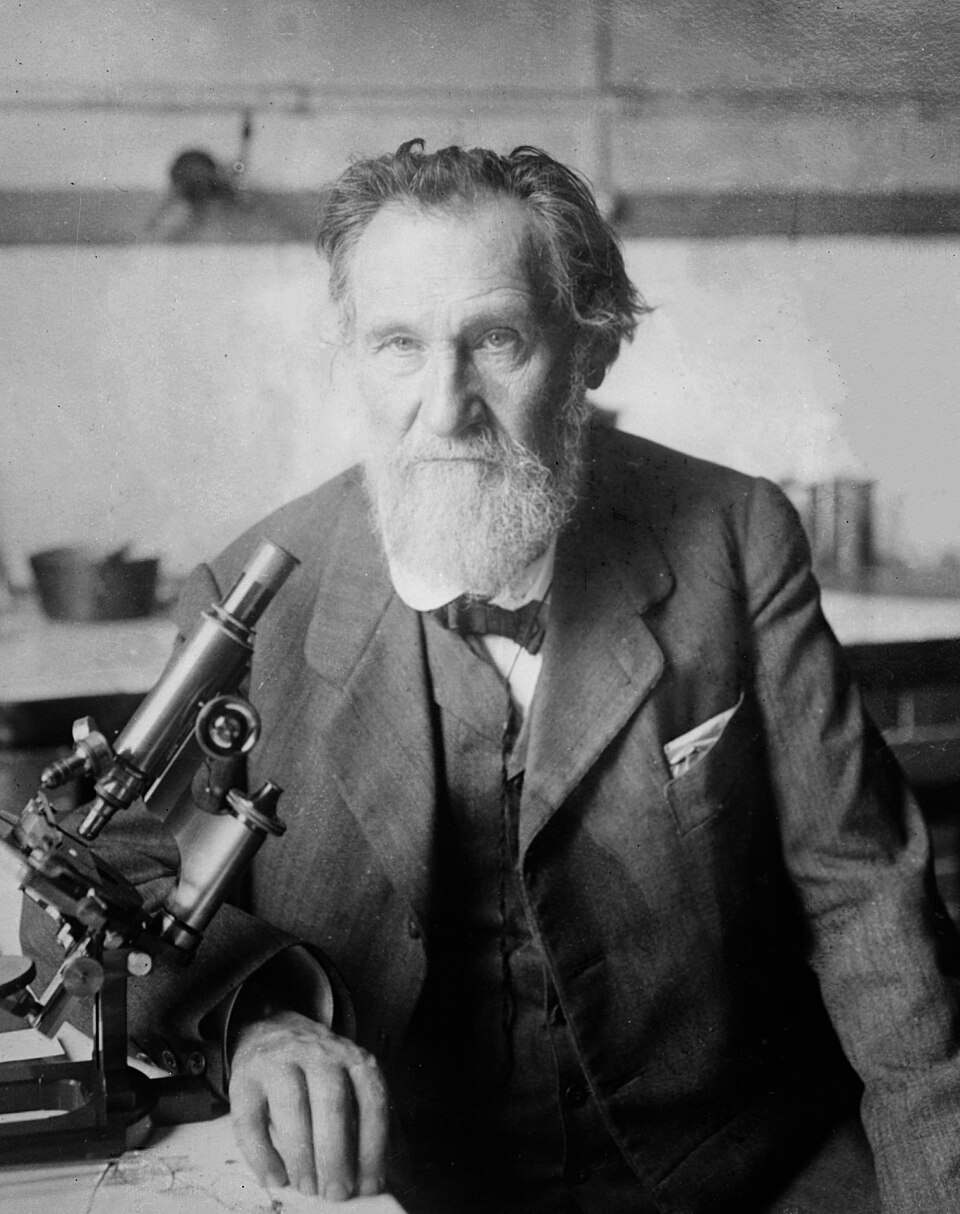
\includegraphics[width=0.30\linewidth]{images/book5/metchnikoff.jpg}\hspace{0.04\linewidth}
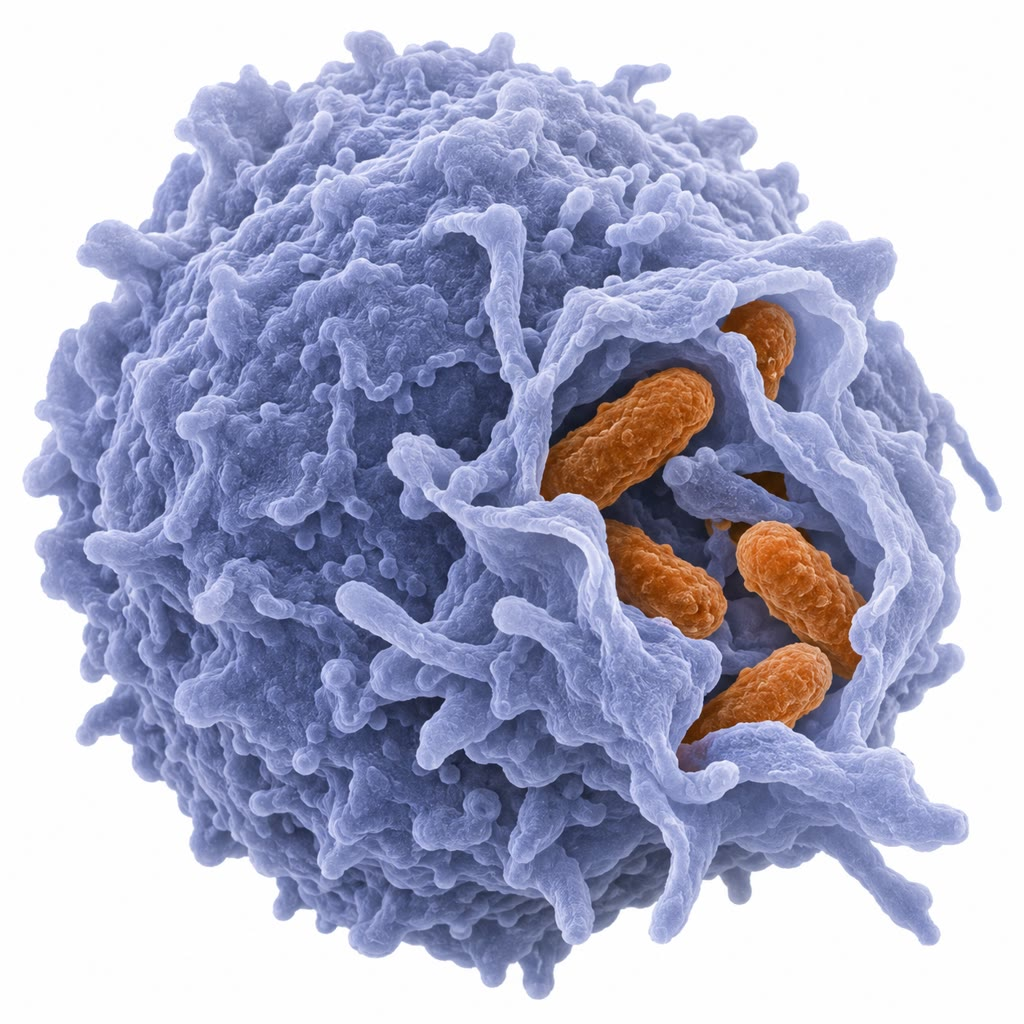
\includegraphics[width=0.30\linewidth]{images/book5/ai/b5-15-neutrophil-phagocytosis.jpg}\hspace{0.04\linewidth}
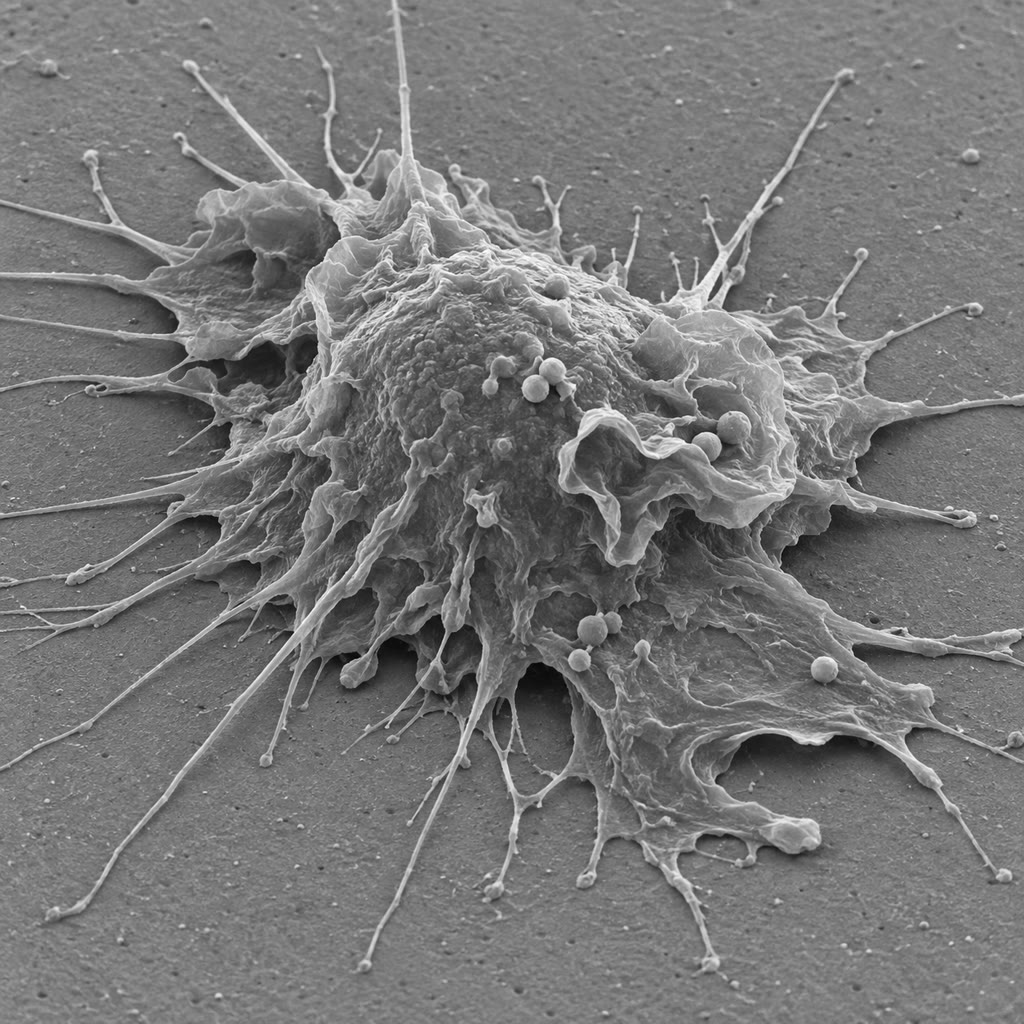
\includegraphics[width=0.30\linewidth]{images/book5/ai/b5-15-macrophage.jpg}

{\small एली मेचनिकॉफ़, जिसने किसी तारामीन-डिंभ में काँटे के चारों ओर
भक्षककोशिकाएँ जुटती देखीं और कोशिकीय प्रतिरक्षा-विज्ञान की नींव रखी
(लाइब्रेरी ऑफ़ कांग्रेस, सार्वजनिक)। बीच में: जीवाणु निगलता कोई
\omterm{def:b3:innate-immunity:innate}{न्यूट्रोफिल}। दाएँ: किसी पृष्ठ पर अपनी झालरदार झिल्लियाँ फैलाता कोई
\omterm{def:b3:innate-immunity:innate}{महाभक्षक}।}
\end{omfigure}

\section{शत्रु को पहचानना}

\begin{definition}[नमूना-पहचान]\label{def:b3:innate-immunity:prr}
\index{नमूना-पहचान ग्राही}\index{रोगजनक-संबद्ध आणविक नमूना}\index{टोल-सदृश ग्राही}\index{क्षति-संबद्ध आणविक नमूना}\index{इन्फ़्लेमासोम}
जन्मजात कोशिकाएँ \emph{रोगजनक-संबद्ध आणविक नमूने} (PAMP) पहचानती हैं:
ऐसे अणु जो सूक्ष्मजीवों के पूरे वर्गों में साझा हैं, उनके लिए अनिवार्य
हैं, और परपोषी में अनुपस्थित --- \omterm{def:b3:bacteriology:envelope}{ग्राम-ऋणात्मक} दीवारों का
\omterm{def:b3:bacteriology:envelope}{लिपोपॉलिसैकेराइड}, \omterm{def:b3:bacteriology:envelope}{ग्राम-धनात्मकों} का पेप्टाइडोग्लाइकन और लिपोटाइकोइक
अम्ल, फ्लैजेलिन, कवकीय $\beta$-ग्लूकन, द्विलड़ी RNA, बिना
5$'$ टोपी का RNA, अमेथिलित \omterm{def:b3:chromatin-epigenetics:methylation}{CpG} वाला DNA, कोशिकाद्रव्य में DNA। ये
ग्राही \emph{नमूना-पहचान ग्राही} (PRR) हैं, कुल मिलाकर कुछ दर्जन, हर
एक किसी एक जीन से कूटबद्ध: पृष्ठ पर और \omterm{def:b3:membrane-traffic:endocytosis}{अंतःकायों} में \emph{टोल-सदृश
ग्राही} (TLR) (\omterm{def:b3:bacteriology:envelope}{लिपोपॉलिसैकेराइड} के लिए TLR4, फ्लैजेलिन के लिए TLR5,
द्विलड़ी RNA के लिए TLR3, \omterm{def:b3:chromatin-epigenetics:methylation}{CpG} DNA के लिए TLR9); पेप्टाइडोग्लाइकन के
टुकड़ों के लिए कोशिकाद्रव्यी NOD प्रोटीन, विषाणुजन्य RNA के लिए RIG-I,
कोशिकाद्रव्यी DNA के लिए cGAS--STING; कवकीय शर्कराओं के लिए
C-प्रकार लेक्टिन। वही ग्राही, या उन्हीं कुलों के दूसरे, आहत कोशिकाओं से
निकले \emph{क्षति-संबद्ध आणविक नमूने} (DAMP) पहचानते हैं --- ATP,
यूरिक अम्ल, केंद्रकीय प्रोटीन HMGB1, सूत्रकणिका DNA --- ताकि बाँझ चोट
भी \omterm{def:b3:innate-immunity:inflammation}{शोथ} पैदा करे। बँधना अनुलेखन कारकों NF-$\kappa$B और इंटरफ़ेरॉन
नियामक कारकों को सक्रिय कर देता है, जो घंटे भर में \omterm{def:b3:innate-immunity:inflammation}{साइटोकाइन},
\omterm{def:b3:innate-immunity:inflammation}{कीमोकाइन}, आसंजन अणु और प्रतिसूक्ष्मजीवी जीन चालू कर देते हैं;
कोशिकाद्रव्यी संवेदकों का एक उपसमुच्चय \emph{इन्फ़्लेमासोम} जोड़ता है,
यानी कोई ऐसा मंच जो कैस्पेज़-1 को सक्रिय करता है ताकि वह
इंटरल्यूकिन-1$\beta$ को उसके सक्रिय रूप में काटे और उस शोथकारी मृत्यु
को छेड़े जिसे पायरोप्टोसिस कहते हैं (\cref{ch:b3:cell-cycle-apoptosis})।
\end{definition}

\begin{proof}[प्रमाण-सामग्री]
जेनवे ने 1989 में प्रस्ताव किया कि अनुकूली प्रतिरक्षा-तंत्र अकेले
प्रतिजन पर अनुक्रिया नहीं देता, बल्कि उसे उन जन्मजात ग्राहियों से कोई
संकेत चाहिए जिन्होंने सूक्ष्मजीवी नमूने पहचाने हों --- यही इसका उत्तर
है कि टीकों को सहवर्धक क्यों चाहिए, ``प्रतिरक्षाविज्ञानी का गंदा छोटा
रहस्य''। हॉफ़मान (1996) ने पाया कि जिन \emph{Drosophila} में ग्राही
टोल न हो --- जो अपनी भ्रूणीय प्रतिरूपण-भूमिका के लिए जाना जाता था ---
वे कोई प्रति-कवकीय अनुक्रिया खड़ी नहीं कर पातीं और फफूँद से ढँकी मर
जाती हैं; ब्यूटलर (1998) ने किसी चूहा-प्रभेद के
लिपोपॉलिसैकेराइड-प्रतिरोध को, जो दूसरों के लिए घातक अंतर्विष-मात्राएँ
झेल जाता था और \omterm{def:b3:bacteriology:envelope}{ग्राम-ऋणात्मक} संक्रमण साफ़ नहीं कर पाता था, स्तनी समजात
TLR4 के किसी उत्परिवर्तन तक मानचित्रित किया। पचास वर्षों से खोजा जा रहा
अंतर्विष का ग्राही कोई टोल था।
\end{proof}

\begin{omfigure}
\begin{tikzpicture}[every node/.style={font=\scriptsize}, >=stealth]
  % membrane
  \draw[very thick, omDef] (0,3.0) -- (11.5,3.0); \draw[very thick, omDef] (0,2.7) -- (11.5,2.7);
  \node[above] at (0.5,3.05) {बाहर}; \node[below] at (0.5,2.65) {कोशिकाद्रव्य};
  % TLR4 with LPS
  \draw[thick, fill=omProp!35] (2.2,2.4) rectangle (2.6,3.9); \draw[thick, fill=omProp!35] (2.9,2.4) rectangle (3.3,3.9);
  \fill[omThm] (2.75,4.1) circle (0.14); \node[above] at (2.75,4.25) {LPS (कोई PAMP)};
  \node[right, align=left] at (3.4,3.5) {MD2 के साथ\\TLR4 द्विलक};
  % signalling
  \node[draw, thick, rounded corners, fill=omDef!20] (myd) at (2.75,1.7) {MyD88, काइनेज़};
  \node[draw, thick, rounded corners, fill=omDef!20] (nfkb) at (2.75,0.6) {NF-$\kappa$B मुक्त};
  \node[draw, thick, rounded corners, fill=omMeth!25, align=center] (genes) at (2.75,-0.8) {TNF, IL-1$\beta$, IL-6, IL-8;\\आसंजन अणु; iNOS};
  \draw[->, thick] (2.75,2.4) -- (myd); \draw[->, thick] (myd) -- (nfkb); \draw[->, thick] (nfkb) -- (genes);
  \node[right, font=\tiny] at (3.3,1.2) {घंटे भर में};
  % cytosolic sensors
  \node[draw, thick, rounded corners, fill=omProp!25, align=center] (rig) at (6.9,1.9) {RIG-I: विषाणुजन्य RNA\\cGAS--STING: कोशिकाद्रव्यी DNA};
  \node[draw, thick, rounded corners, fill=omMeth!25] (ifn) at (6.9,-0.2) {प्ररूप~I इंटरफ़ेरॉन};
  \draw[->, thick] (rig) -- node[midway, right] {IRF3, IRF7} (ifn);
  \node[draw, thick, rounded corners, fill=omThm!20, align=center] (nlrp) at (10.9,1.9) {NLRP3 इन्फ़्लेमासोम:\\क्रिस्टल, ATP, छिद्र};
  \node[draw, thick, rounded corners, fill=omMeth!25, align=center] (il1) at (10.9,-0.8) {कैस्पेज़-1: IL-1$\beta$\\मुक्त; पायरोप्टोसिस};
  \draw[->, thick] (nlrp) -- (il1);
  \draw[->, thick, dashed] (genes.south) -- ++(0,-0.5) -| (il1.south) node[pos=0.25, below, font=\tiny] {TLR पथ से जुटा पूर्व-IL-1$\beta$};
\end{tikzpicture}

{\small नमूना-पहचान की तीन भुजाएँ। \omterm{def:b3:bacteriology:envelope}{लिपोपॉलिसैकेराइड} से बँधा कोई पृष्ठीय
\omterm{def:b3:innate-immunity:prr}{टोल-सदृश ग्राही} NF-$\kappa$B के ज़रिए शोथकारी \omterm{def:b3:innate-immunity:inflammation}{साइटोकाइनों} तक संकेत
भेजता है; विषाणुजन्य न्यूक्लिक अम्ल के कोशिकाद्रव्यी संवेदक इंटरफ़ेरॉन
प्रेरित करते हैं; और \omterm{def:b3:innate-immunity:prr}{इन्फ़्लेमासोम} इंटरल्यूकिन-1 के संचित पूर्ववर्ती को
सक्रिय \omterm{def:b3:innate-immunity:inflammation}{साइटोकाइन} में बदल देता है।}
\end{omfigure}

\begin{definition}[पूरक तंत्र]\label{def:b3:innate-immunity:complement}
\index{पूरक तंत्र}\index{C3 कन्वर्टेज़}\index{ऑप्सोनीकरण}\index{झिल्ली-आक्रमण संकुल}\index{ऐनाफ़ाइलोटॉक्सिन}
\emph{पूरक तंत्र} कोई तीस प्लाज़्मा प्रोटीनों का तंत्र है, यानी सीरम
ग्लोब्युलिनों का \qty{10}{\%}, जो प्रोटीन-अपघटनी सक्रियणों की किसी
शृंखला से सूक्ष्मजीवों को चिह्नित और नष्ट करता है। तीन पथ केंद्रीय
प्रोटीन C3 के विदलन पर मिलते हैं: \emph{चिरप्रतिष्ठित} पथ, जो किसी
पृष्ठ पर बैठे प्रतिरक्षियों (या \omterm{prop:b3:innate-immunity:systemic}{C-क्रियाशील प्रोटीन}, या एपॉप्टोटिक
कोशिकाओं) से C1q के बँधने पर शुरू होता है; \emph{लेक्टिन} पथ, जो
सूक्ष्मजीवी शर्कराएँ पहचानते मैनोस-बंधक लेक्टिन से शुरू होता है; और
\emph{वैकल्पिक} पथ, जिसमें C3 किसी कम दर से स्वतः जल-अपघटित होता है और
उससे बना C3b जिस भी पृष्ठ से मिले उससे चिपक जाता है। हर पथ कोई
\emph{C3 कन्वर्टेज़} बनाता है, यानी वह एंज़ाइम जो और C3 काटती है; जो
C3b वह पृष्ठ पर सहसंयोजी रूप से जमाती है वह बदले में और कन्वर्टेज़ बना
देता है --- कोई प्रवर्धन-पाश --- जिससे कोई जीवाणु मिनटों में लाखों C3b
से ढँक जाता है। C3b कोई \emph{ऑप्सोनिन} है: भक्षककोशिकाएँ उसके ग्राही
ढोती हैं और जिसे वह ढँके उसे खा जाती हैं। छोटे टुकड़े C3a और C5a
\emph{ऐनाफ़ाइलोटॉक्सिन} हैं, जो वाहिकाएँ फैलाते हैं, \omterm{def:b3:innate-immunity:innate}{न्यूट्रोफिल}
खींचते हैं और मास्ट कोशिकाएँ सक्रिय करते हैं। और C5b, C6--C9 को जोड़कर
\emph{झिल्ली-आक्रमण संकुल} बनाता है, यानी \qty{10}{nm} का कोई छिद्र, जो
\omterm{def:b3:bacteriology:envelope}{ग्राम-ऋणात्मक} जीवाणुओं और परिवेष्टित \omterm{def:b3:virology:virus}{विषाणुओं} का लयन कर देता है।
परपोषी कोशिकाएँ इसलिए बच जाती हैं कि वे नियामक ढोती हैं --- कारक~H,
CD55, CD59 --- जो अपने ही पृष्ठों पर कन्वर्टेज़ तोड़ देते हैं और वह
छिद्र रोक देते हैं; सूक्ष्मजीव, जिनके पास वे नहीं, उस पाश के हवाले हो
जाते हैं।
\end{definition}

\begin{theorem}[गतिक विभेदक के रूप में पूरक-पाश]\label{thm:b3:innate-immunity:complement}
\index{पूरक तंत्र!प्रवर्धन-पाश}
मान लीजिए $B(t)$ किसी पृष्ठ पर जमे C3b अणुओं की संख्या है। C3 की
स्वतःचाल से C3b किसी छोटी अचर दर $k_{0}$ पर जमता है, और हर जमा हुआ
C3b ऐसी कन्वर्टेज़ बनाता है जो प्रति C3b प्रति सेकंड दर $a$ पर और जमाती
है, जबकि नियामक (परपोषी) और क्षय कन्वर्टेज़ की क्रियाशीलता प्रति C3b
प्रति सेकंड दर $d$ पर हटाते हैं:
\[
\frac{\mathrm{d}B}{\mathrm{d}t} = k_{0} + (a - d)\,B .
\]
जिस पृष्ठ पर $a > d$ हो --- कोई सूक्ष्मजीव, जिसके पास नियामक नहीं ---
वहाँ $B(t) = \bigl[k_{0}/(a-d)\bigr]\bigl(e^{(a-d)t} - 1\bigr)$ काल-अचर
$1/(a - d)$ के साथ चरघातांकी रूप से बढ़ता है; किसी परपोषी पृष्ठ पर,
जहाँ $d > a$ है, $B$ छोटे स्थायी मान $k_{0}/(d - a)$ के पास पहुँचता
है। वही अणु, उन्हीं सांद्रताओं पर, कुछ मिनटों में किसी जीवाणु पर दस
लाख C3b जमा देते हैं और उसके बगल की कोशिका पर कुछ दर्जन: स्व और पर का
भेद पहचान से नहीं, बल्कि $a - d$ के चिह्न से होता है।
\end{theorem}
\begin{proof}
यह समीकरण अचर गुणांकों वाला रैखिक समीकरण है। $a \ne d$ के लिए स्थिर
बिंदु $B^{*} = -k_{0}/(a-d)$ है; $B = B^{*} + u$ लिखने पर
$\mathrm{d}u/\mathrm{d}t = (a-d)u$, इसलिए $u = u_{0}e^{(a-d)t}$, और
$B(0) = 0$ के साथ $B(t) = \bigl[k_{0}/(a-d)\bigr](e^{(a-d)t} - 1)$। $a > d$
के लिए यह बिना किसी सीमा के बढ़ता है (जब तक C3 या पृष्ठ चुक न जाए);
$a < d$ के लिए वह चरघातांक क्षीण होता है और $B \to k_{0}/(d-a) > 0$।
प्रति सेकंड $k_{0} = 1$ और किसी जीवाणु पर $a - d = \qty{0.1}{s^{-1}}$
के साथ $B(\qty{2}{min})
= 10(e^{12} - 1) \approx 1.6\times 10^{6}$; किसी परपोषी कोशिका पर $d - a =
\qty{0.1}{s^{-1}}$ के साथ $B^{*} = 10$।
\end{proof}

\begin{omfigure}
\begin{tikzpicture}
\begin{axis}[
  width=0.66\linewidth, height=5.6cm,
  axis x line=bottom, axis y line=left,
  xmin=0, xmax=150, ymin=1, ymax=1e7, ymode=log,
  xlabel={सेकंड}, ylabel={जमा C3b},
  xlabel style={font=\small, at={(axis description cs:0.5,-0.12)}, anchor=north}, ylabel style={font=\small},
  tick label style={font=\small}, xtick={0,30,60,90,120,150},
  clip=false,
]
\addplot[very thick, omThm, domain=1:150, samples=80] {10*(exp(0.1*x)-1)};
\addplot[very thick, omDef, domain=1:150, samples=80] {10*(1-exp(-0.1*x))};
\node[font=\scriptsize, omThm, anchor=east] at (axis cs:100,2e5) {सूक्ष्मजीव: $a > d$, चरघातांकी};
\node[font=\scriptsize, omDef, anchor=south west] at (axis cs:60,14) {परपोषी कोशिका: $d > a$, $k_{0}/(d-a)$ पर संतृप्त};
\end{axis}
\end{tikzpicture}

{\small दो पृष्ठों पर पूरक-पाश, प्रति सेकंड $k_{0} = 1$ और
$|a - d| = \qty{0.1}{s^{-1}}$ के साथ: नियामकों से रहित किसी
सूक्ष्मजीव पर C3b चरघातांकी रूप से बढ़ता है और दो मिनटों में दस लाख तक
पहुँचता है; नियामकों वाली किसी परपोषी कोशिका पर वह दस पर ठहर जाता है।}
\end{omfigure}

\begin{omfigure}
\begin{tikzpicture}[every node/.style={font=\scriptsize}, >=stealth]
  \node[draw, thick, rounded corners, fill=omDef!20, align=center] (cl) at (-4.2,3.0) {चिरप्रतिष्ठित:\\प्रतिरक्षी या C-क्रियाशील\\प्रोटीन पर C1q};
  \node[draw, thick, rounded corners, fill=omDef!20, align=center] (le) at (0,3.0) {लेक्टिन:\\सूक्ष्मजीवी शर्कराओं पर\\मैनोस-बंधक लेक्टिन};
  \node[draw, thick, rounded corners, fill=omDef!20, align=center] (al) at (4.2,3.0) {वैकल्पिक:\\स्वतःस्फूर्त C3 स्वतःचाल,\\किसी भी पृष्ठ पर C3b};
  \node[draw, thick, rounded corners, fill=omProp!35, minimum width=3cm] (conv) at (0,1.2) {C3 कन्वर्टेज़};
  \node[draw, thick, rounded corners, fill=omThm!25, align=center] (c3b) at (0,-0.4) {C3 $\to$ C3b (पृष्ठ पर) $+$ C3a};
  \draw[->, thick] (cl) -- (conv); \draw[->, thick] (le) -- (conv); \draw[->, thick] (al) -- (conv);
  \draw[->, thick] (conv) -- (c3b);
  \draw[->, very thick, omThm] (c3b.east) .. controls (3.2,-0.4) and (3.2,1.2) .. (conv.east) node[pos=0.5, right, align=left] {प्रवर्धन-पाश:\\C3b और कन्वर्टेज़ बनाता है};
  \node[draw, thick, rounded corners, fill=omMeth!25, align=center] (ops) at (-4.4,-2.2) {ऑप्सोनीकरण:\\C3b जिसे ढँके उसे\\भक्षककोशिकाएँ खाती हैं};
  \node[draw, thick, rounded corners, fill=omMeth!25, align=center] (ana) at (0,-2.2) {C3a, C5a:\\वाहिकाएँ फैलतीं, न्यूट्रोफिल\\और मास्ट कोशिकाएँ बुलायी जातीं};
  \node[draw, thick, rounded corners, fill=omMeth!25, align=center] (mac) at (4.4,-2.2) {C5b--C9:\\झिल्ली-आक्रमण संकुल,\\लयन};
  \draw[->, thick] (c3b) -- (ops); \draw[->, thick] (c3b) -- (ana); \draw[->, thick] (c3b) -- (mac);
  \node[draw, thick, rounded corners, fill=gray!15, align=center] (reg) at (-4.4,1.2) {परपोषी नियामक:\\कारक~H, CD55, CD59};
  \draw[-|, thick, gray!60!black] (reg) -- (conv);
\end{tikzpicture}

{\small \omterm{def:b3:innate-immunity:complement}{पूरक तंत्र}। तीन रास्ते कोई \omterm{def:b3:innate-immunity:complement}{C3 कन्वर्टेज़} बनाते हैं; जो C3b वह
जमाती है वह और कन्वर्टेज़ बना देता है (प्रमेय का पाश), और जमा C3b
\omterm{def:b3:innate-immunity:complement}{ऑप्सोनीकरण} करता है, टुकड़े \omterm{def:b3:innate-immunity:inflammation}{शोथ} पैदा करते हैं, और अंतिम संकुल लयन।
परपोषी कोशिकाएँ ऐसे नियामक ढोती हैं जो अपनी ही झिल्लियों पर वह पाश काट
देते हैं (और, CD59 के साथ, वह छिद्र रोक देते हैं)।}
\end{omfigure}

\section{शोथ}

\begin{definition}[तीव्र शोथ]\label{def:b3:innate-immunity:inflammation}
\index{शोथ}\index{साइटोकाइन}\index{कीमोकाइन}\index{वाहिका-निर्गमन}\index{सिलेक्टिन}\index{इंटिग्रिन}
\emph{शोथ} चोट या संक्रमण के प्रति वाहिकामय ऊतक की अनुक्रिया है, जिसका
संचालन \emph{साइटोकाइन} करते हैं --- प्रतिरक्षा कोशिकाओं के वे छोटे
संकेतक प्रोटीन, यहाँ मुख्यतः सक्रिय \omterm{def:b3:innate-immunity:innate}{महाभक्षकों} से आते TNF,
इंटरल्यूकिन-1 और इंटरल्यूकिन-6 --- और \emph{कीमोकाइन}, यानी वे
साइटोकाइन जो प्रवासन की दिशा तय करते हैं। उसके चरण सेल्सस के चिह्नों की
व्याख्या कर देते हैं। मास्ट कोशिकाओं से आता हिस्टामिन, नाइट्रिक
ऑक्साइड और प्रोस्टाग्लैंडिन अणुधमनियाँ फैलाते हैं: \emph{लाली} और
\emph{ऊष्मा}। अणुशिराओं का अंतःस्तर सिकुड़ता है और प्लाज़्मा रिसने देता
है, जिसके प्रोटीन --- पूरक, प्रतिरक्षी, स्कंदन कारक --- ऊतक में भर
जाते हैं: \emph{सूजन}। ब्रैडीकाइनिन और प्रोस्टाग्लैंडिन E$_{2}$
तंत्रिका-सिरे संवेदी बना देते हैं: \emph{पीड़ा}। और श्वेताणु
\emph{वाहिका-निर्गमन} से पहुँचते हैं: TNF तथा इंटरल्यूकिन-1 अंतःस्तर
से \emph{सिलेक्टिन} प्रदर्शित करवाते हैं, जिन पर गुज़रते \omterm{def:b3:innate-immunity:innate}{न्यूट्रोफिल}
अटकते और लुढ़कते हैं; अंतःस्तरी पृष्ठ पर बैठे कीमोकाइन
(इंटरल्यूकिन-8) \omterm{def:b3:innate-immunity:innate}{न्यूट्रोफिलों} के \emph{इंटिग्रिन} सक्रिय कर देते हैं,
जो अंतःस्तरी आसंजन अणुओं से कसकर बँधते हैं और कोशिका रोक देते हैं; और
\omterm{def:b3:innate-immunity:innate}{न्यूट्रोफिल} अंतःस्तरी कोशिकाओं के बीच से निचुड़कर कीमोकाइन-प्रवणता के
सहारे ऊतक में चला जाता है --- यह पूरा क्रम कुछ मिनटों में, किसी
संक्रमित स्थल में प्रति घंटे दस लाख कोशिकाओं तक की दर से।
\end{definition}

\begin{omfigure}
\begin{tikzpicture}[every node/.style={font=\scriptsize}, >=stealth]
  % vessel wall
  \fill[omThm!10] (0,0) rectangle (12,2.3); \node[left, omThm!70!black, anchor=north east] at (12,2.25) {रक्त, बहता हुआ $\rightarrow$};
  \foreach \x in {0,1.5,3,4.5,6,7.5,9,10.5} \draw[thick, fill=omDef!30] (\x,-0.05) rectangle (\x+1.45,0.35);
  \node[right] at (0.1,-0.35) {अंतःस्तर};
  \fill[omMeth!8] (0,-1.7) rectangle (12,-0.45); \node[right, omMeth!60!black] at (0.1,-1.55) {ऊतक};
  % bacteria and chemokine gradient
  \foreach \p in {(10.6,-1.1),(11.0,-0.9),(11.3,-1.2)} \fill[omProp] \p ellipse (0.14 and 0.07);
  \node[below, omProp] at (11.0,-1.35) {जीवाणु};
  \node[below, font=\tiny] at (8.0,-0.5) {कीमोकाइन-प्रवणता $\rightarrow$};
  % neutrophils in sequence
  \draw[thick, fill=white] (1.2,1.1) circle (0.3); \node[above] at (1.2,1.45) {1. बहता};
  \draw[thick, fill=white] (3.4,0.68) circle (0.3); \node[above] at (3.4,1.05) {2. सिलेक्टिनों पर लुढ़कता};
  \draw[omThm, thick] (3.1,0.45) -- (3.05,0.35); \draw[omThm, thick] (3.4,0.38) -- (3.4,0.35); \draw[omThm, thick] (3.7,0.45) -- (3.75,0.35);
  \draw[thick, fill=white] (6.0,0.62) ellipse (0.38 and 0.26); \node[above, align=center] at (6.0,0.95) {3. दृढ़ आसंजन\\(इंटिग्रिन)};
  \draw[thick, fill=white] (8.25,0.18) ellipse (0.2 and 0.42); \node[above, align=center] at (8.4,0.95) {4. बीच से\\निचुड़ना};
  \draw[thick, fill=white] (9.6,-1.0) circle (0.3); \node[left] at (9.25,-1.0) {5. स्थल की ओर रेंगना};
  \draw[->, thick, gray] (1.5,1.05) -- (3.0,0.8); \draw[->, thick, gray] (3.7,0.68) -- (5.6,0.62); \draw[->, thick, gray] (6.4,0.5) -- (8.0,0.4); \draw[->, thick, gray] (8.3,-0.3) -- (9.3,-0.8);
  % TNF label
  \node[below, align=center, font=\tiny] at (4.0,-1.75) {ऊतक-महाभक्षकों से आते TNF और IL-1 अंतःस्तर से वे सिलेक्टिन\\और आसंजन अणु प्रदर्शित करवाते हैं जो न्यूट्रोफिलों को पकड़ लेते हैं};
\end{tikzpicture}

{\small \omterm{def:b3:innate-immunity:inflammation}{वाहिका-निर्गमन}। \omterm{def:b3:innate-immunity:innate}{ऊतक-महाभक्षकों} से आते \omterm{def:b3:innate-immunity:inflammation}{साइटोकाइन} अणुशिरा की
दीवार चिपचिपी कर देते हैं; कोई गुज़रता \omterm{def:b3:innate-immunity:innate}{न्यूट्रोफिल} \omterm{def:b3:innate-immunity:inflammation}{सिलेक्टिनों} पर अटककर
लुढ़कता है, अपने \omterm{def:b3:innate-immunity:inflammation}{इंटिग्रिनों} से रोका जाता है, अंतःस्तरी कोशिकाओं के बीच
से निचुड़ता है, और कीमोकाइन-प्रवणता के सहारे जीवाणुओं तक जाता है।}
\end{omfigure}

\begin{proposition}[ज्वर, तीव्र प्रावस्था और शमन]\label{prop:b3:innate-immunity:systemic}
\index{ज्वर}\index{तीव्र-प्रावस्था अनुक्रिया}\index{C-क्रियाशील प्रोटीन}\index{शोथ का शमन}
इंटरल्यूकिन-1, TNF और इंटरल्यूकिन-6 दूर बैठे भी काम करते हैं।
अधश्चेतक में वे प्रोस्टाग्लैंडिन E$_{2}$ प्रेरित करते हैं, जो शरीर के
तापमान का नियत बिंदु उठा देता है: \emph{ज्वर}, जो अनेक जीवाणु धीमे कर
देता है, प्रतिरक्षा कोशिकाओं की अपनी अभिक्रियाएँ तेज़ करता है, और प्रति
अंश उपापचय पर लगभग \qty{12}{\%} अधिक लागत लेता है। यकृत में वे
\emph{तीव्र-प्रावस्था प्रोटीन} प्रेरित करते हैं --- \omterm{prop:b3:innate-immunity:systemic}{C-क्रियाशील
प्रोटीन}, जो जीवाणुओं का फ़ॉस्फ़ोकोलीन बाँधता है, पूरक सक्रिय करता है और
दो दिनों में हज़ार गुना चढ़ जाता है, यानी चिकित्सक का शोथ-माप;
फ़ाइब्रिनोजन; मैनोस-बंधक लेक्टिन; और हेप्सिडिन, जो लोहे को उन
सूक्ष्मजीवों से दूर बंद कर देता है जिन्हें वह चाहिए। मज्जा में वे
\omterm{def:b3:innate-immunity:innate}{न्यूट्रोफिल} छोड़ते हैं और उनका उत्पादन तेज़ करते हैं। \omterm{def:b3:innate-immunity:inflammation}{शोथ} का अंत होना
ही चाहिए: जैसे-जैसे उद्दीपक साफ़ होता है, लिपिड मध्यस्थ
प्रोस्टाग्लैंडिनों से लिपॉक्सिनों और रिज़ॉल्विनों की ओर बदल जाते हैं,
\omterm{def:b3:innate-immunity:innate}{न्यूट्रोफिल} \omterm{def:b3:cell-cycle-apoptosis:apoptosis}{एपॉप्टोसिस} से मरते हैं और \omterm{def:b3:innate-immunity:innate}{महाभक्षकों} द्वारा खाए जाते हैं,
जो फिर किसी मरम्मत-कार्यक्रम पर चले जाते हैं और वृद्धि कारक तथा
इंटरल्यूकिन-10 स्रवित करते हैं --- यही \emph{शमन} है। जब उद्दीपक बना
रहे (कोई तपेदिक-दंडाणु जो मारा न जा सके, कोई क्रिस्टल, कोई स्व-प्रतिजन)
तब अनुक्रिया चिरकारी हो जाती है: \omterm{def:b3:innate-immunity:innate}{महाभक्षक} उस स्थल को किसी कणिकागुल्म
में चुन देते हैं, तंतुकोरक व्रणचिह्न बिछा देते हैं, और ऊतक अपने ही बचाव
से नष्ट हो जाता है।
\end{proposition}

\begin{example}[पूतिता]\label{ex:b3:innate-immunity:sepsis}
किसी किरच तक सीमित \omterm{def:b3:innate-immunity:inflammation}{शोथ} कोई इलाज है; वही अभिक्रियाएँ पूरे शरीर में कोई
महाविपत्ति। जब जीवाणु या उनका \omterm{def:b3:bacteriology:envelope}{लिपोपॉलिसैकेराइड} बड़ी मात्रा में रक्त तक
पहुँचें, तब हर जगह के \omterm{def:b3:innate-immunity:innate}{महाभक्षक} एक साथ TNF और इंटरल्यूकिन-1 छोड़ते हैं:
हर वाहिका फैलती और रिसती है, रक्तचाप ढह जाता है, दस हज़ार केशिकाओं में
स्कंदन सक्रिय होकर स्कंदन कारक चुका देता है, और अंग, सिंचन से वंचित,
विफल हो जाते हैं --- यही \emph{पूतिजन्य आघात} है, जो अपने चौथाई से आधे
शिकारों को मार देता है, यानी साल में कोई एक करोड़ दस लाख लोग।
किसी स्वयंसेवक में अंतःक्षिप्त कुछ माइक्रोग्राम \omterm{def:b3:bacteriology:envelope}{लिपोपॉलिसैकेराइड} दो
घंटों के भीतर ज्वर, कँपकँपी और रक्तचाप की गिरावट पैदा कर देते हैं; और
जिस चूहे में TLR4 न हो वह सौ गुना घातक मात्रा झेल जाता है। रोग परपोषी
की अपनी अनुक्रिया है, और जो \omterm{def:b3:bacteriology:antibiotics}{प्रतिजैविक} जीवाणु मारते हैं वे कुछ घंटों
के लिए और अंतर्विष छोड़कर उसे बदतर कर सकते हैं।
\end{example}

\begin{omfigure}
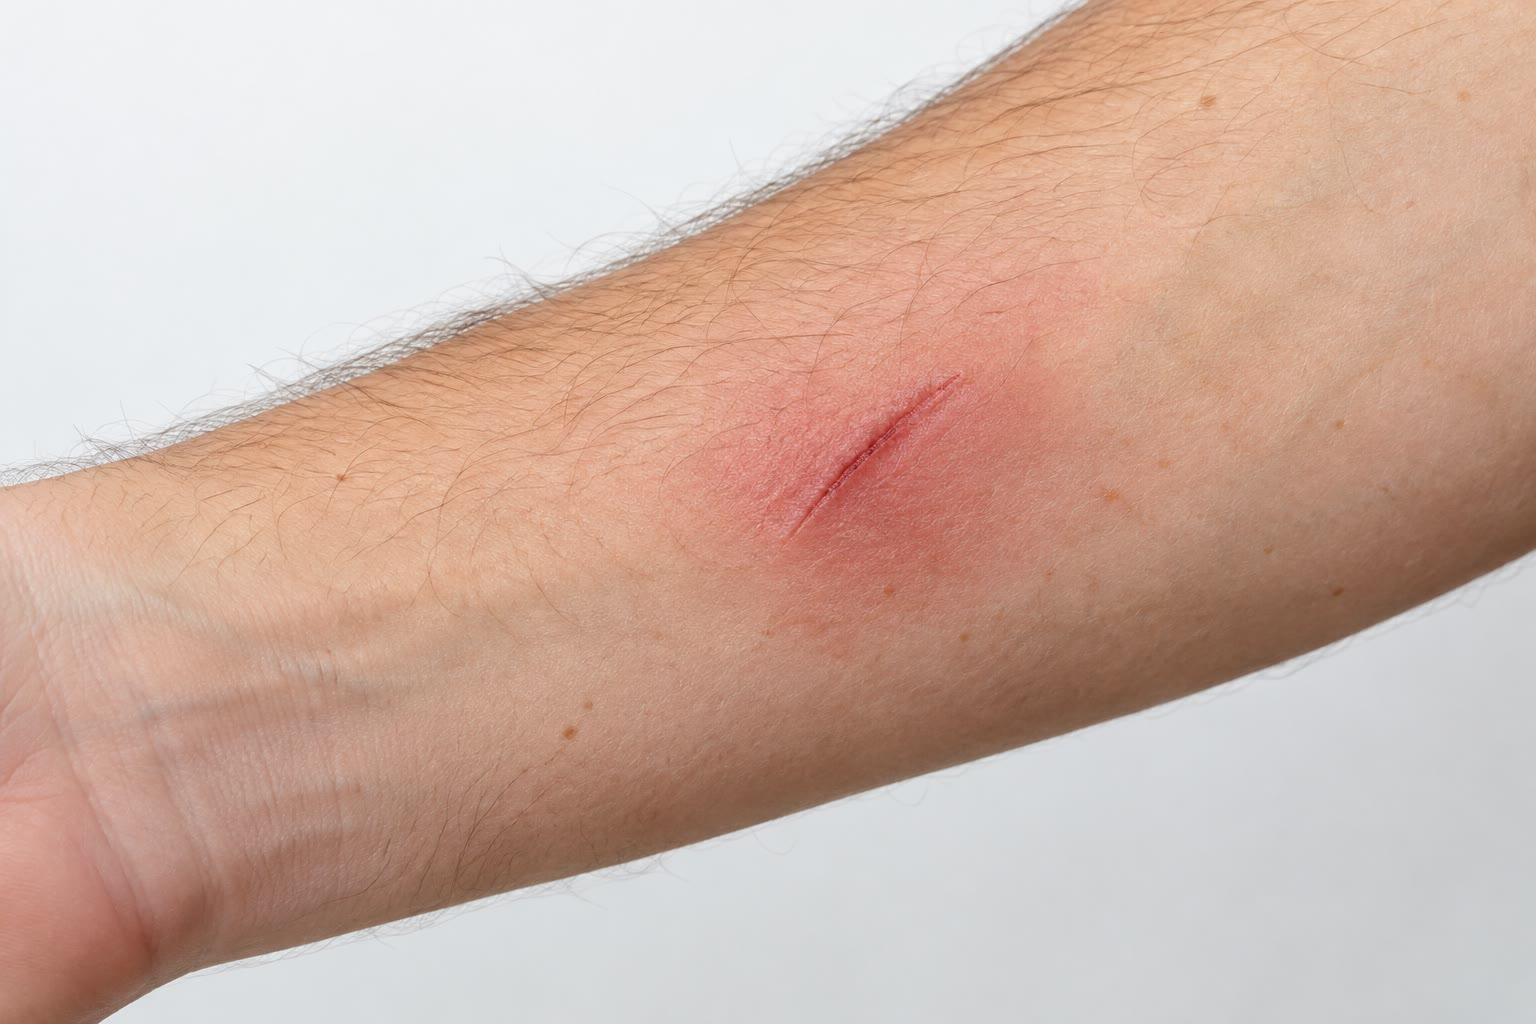
\includegraphics[width=0.52\linewidth]{images/book5/ai/b5-15-inflamed-skin.jpg}

{\small काँटे की खरोंच के चारों ओर तीव्र \omterm{def:b3:innate-immunity:inflammation}{शोथ}: फैली वाहिकाओं से लाली और
गरमाहट, रिसे प्लाज़्मा से सूजन, और वह पीड़ा जो अंग को हिलने नहीं देती
--- वही स्थानीय अनुक्रिया, जो पूरे शरीर तक फैल जाए तो पूतिजन्य आघात
है।}
\end{omfigure}

\section{मारना}

\begin{definition}[भक्षण और श्वसन-विस्फोट]\label{def:b3:innate-immunity:killing}
\index{भक्षण}\index{श्वसन-विस्फोट}\index{NADPH ऑक्सिडेज़}\index{न्यूट्रोफिल बाह्यकोशिकीय जाल}
कोई भक्षककोशिका अपने शिकार को ऑप्सोनिनों के ग्राहियों से --- C3b, और
प्रतिरक्षियों के अचर क्षेत्र --- या सीधे नमूना-ग्राहियों से बाँधती है,
उसे झिल्ली में लपेटती है, और \emph{भक्षकाय} बंद कर देती है, जो कणिकाओं
तथा \omterm{def:b3:membrane-traffic:endocytosis}{लयनकायों} से संलयित होता है। मारना एक साथ कई उपायों से होता है।
\emph{श्वसन-विस्फोट}: भक्षकाय-झिल्ली पर जुड़ी वह एंज़ाइम
\emph{NADPH ऑक्सिडेज़} इलेक्ट्रॉन ऑक्सीजन पर पंप करके सुपरऑक्साइड
बनाती है, जो हाइड्रोजन परॉक्साइड बन जाता है, जिसे मायलोपेरॉक्सिडेज़,
क्लोराइड के साथ, हाइपोक्लोराइट में बदल देती है --- यानी ब्लीच, किसी
माइक्रोमीटर चौड़े कक्ष के भीतर मिलीमोलर सांद्रता पर। प्रेरणीय NO
संश्लेषेज़ से नाइट्रिक ऑक्साइड, जो सुपरऑक्साइड के साथ परॉक्सीनाइट्राइट
देता है। अम्ल, pH~5 तक। लाइसोज़ाइम, प्रोटीएज़, लैक्टोफ़ेरिन जो शिकार को
लोहे से वंचित कर देता है, और डिफ़ेंसिन जो उसे छेद देते हैं। जो
\omterm{def:b3:innate-immunity:innate}{न्यूट्रोफिल} अपने मिले शिकार को खा न सके --- कोई कवक-तंतु, कोई गुच्छा
--- वह अपना ही \omterm{def:b3:chromatin-epigenetics:nucleosome}{क्रोमैटिन} DNA तथा कणिका-प्रोटीनों के किसी चिपचिपे जाल के
रूप में बाहर फेंक सकता है, यानी कोई \emph{\omterm{def:b3:innate-immunity:innate}{न्यूट्रोफिल} बाह्यकोशिकीय
जाल}, और ऐसा करते हुए मर सकता है। जिन बच्चों को दोषपूर्ण NADPH
ऑक्सिडेज़ विरासत में मिले (चिरकारी कणिकागुल्मी रोग) वे उन्हीं जीवाणुओं
और कवकों से बार-बार लौटते फोड़े तथा कणिकागुल्म झेलते हैं जिन्हें
साधारण भक्षककोशिकाएँ बिना कठिनाई मार देती हैं: वह विस्फोट वैकल्पिक
नहीं है।
\end{definition}

\begin{definition}[प्राकृतिक घातक कोशिकाएँ और इंटरफ़ेरॉन]\label{def:b3:innate-immunity:nk-ifn}
\index{प्राकृतिक घातक कोशिका!अनुपस्थित स्व}\index{इंटरफ़ेरॉन!प्ररूप~I}\index{प्रति-विषाणु अवस्था}
\omterm{def:b3:virology:virus}{विषाणु} कोशिकाओं के भीतर छिपते हैं, जहाँ पूरक और भक्षककोशिकाएँ उन तक
नहीं पहुँच सकतीं। \emph{\omterm{def:b3:innate-immunity:innate}{प्राकृतिक घातक कोशिकाएँ}} उन कोशिकाओं की गश्त
लगाती हैं जिन्होंने MHC वर्ग~I दिखाना बंद कर दिया हो --- किसी ऐसी
कोशिका का ``अनुपस्थित स्व'' जिसके विषाणुजन्य या अर्बुदीय निवासी ने
T~कोशिकाओं से बचने के लिए प्रतिजन-प्रस्तुति बंद कर दी हो
(\cref{ch:b3:adaptive-immunity}) --- और उन दबाव-प्रोटीनों की भी जिन्हें
संक्रमित तथा रूपांतरित कोशिकाएँ अपने पृष्ठ पर लगा देती हैं; MHC~I के
निरोधी ग्राही और दबाव-बंधकों के सक्रियकारी ग्राही जोड़े जाते हैं, और
जो कोशिका पलड़ा झुका दे वह मिनटों के भीतर उसमें अंतःक्षिप्त परफ़ोरिन तथा
ग्रैन्ज़ाइमों से मार दी जाती है, जो उसका \omterm{def:b3:cell-cycle-apoptosis:apoptosis}{एपॉप्टोसिस} छेड़ देते हैं।
\emph{प्ररूप~I इंटरफ़ेरॉन} ($\alpha$ और $\beta$) हर उस कोशिका से बनते
हैं जिसके RIG-I या cGAS ने विषाणुजन्य न्यूक्लिक अम्ल पकड़ा हो; स्रवित
होकर वे पड़ोसी कोशिकाओं के ग्राहियों से बँधते हैं और, JAK--STAT पथ के
ज़रिए, सैकड़ों जीन प्रेरित करते हैं जो उन कोशिकाओं को किसी
\emph{प्रति-विषाणु अवस्था} में डाल देते हैं: कोई ऐसी काइनेज़ जो द्विलड़ी
RNA मिलते ही अनुवादन बंद कर देती है, कोई न्यूक्लिएज़ जो RNA का अपघटन
करती है, ऐसे प्रोटीन जो \omterm{def:b3:virology:virus}{विषाणु} का प्रवेश और संयोजन रोकते हैं, और और भी
MHC~I ताकि T~कोशिकाओं को भीतर का हाल दिखे। जिस कोशिका ने इंटरफ़ेरॉन
बनाया वह शायद मर जाए; उसके पड़ोसी पहले से चेता दिए जाते हैं। इंटरफ़ेरॉन
की खोज आइज़ैक्स और लिंडनमान (1957) ने विषाणु-संक्रमित कोशिकाओं के माध्यम
में उस कारक के रूप में की जो ताज़ा कोशिकाओं को प्रतिरोधी बना देता था,
और वही कारण है कि एक \omterm{def:b3:virology:virus}{विषाणु} से संक्रमित कोई कोशिका दूसरे का प्रतिरोध
करती है।
\end{definition}

\begin{method}[शोथ और भक्षककोशिका-प्रकार्य नापना]\label{met:b3:innate-immunity:tests}
\index{C-क्रियाशील प्रोटीन!परीक्षण}\index{नाइट्रोब्लू टेट्राज़ोलियम परीक्षण}
रोगी की शय्या पर: (1) सीरम में \emph{\omterm{prop:b3:innate-immunity:systemic}{C-क्रियाशील प्रोटीन}},
प्रतिरक्षा-परीक्षण से --- विश्राम में \qty{5}{mg/L} से नीचे, किसी
\omterm{def:b3:virology:virus}{विषाणु} संक्रमण में दहाई में, जीवाणुजन्य पूतिता में सैकड़ों में, और
प्रभावी उपचार के दिनों के भीतर गिरता हुआ; (2) न्यूट्रोफिल-गणना, जो
जीवाणु संक्रमण में चढ़ती है और जिसमें अपरिपक्व रूप मज्जा से जल्दी छोड़
दिए जाते हैं; (3) लोहिताणु अवसादन दर, जो फ़ाइब्रिनोजन का कोई धीमा
प्रतिनिधि है। भक्षककोशिकाओं के लिए: (4) \emph{नाइट्रोब्लू
टेट्राज़ोलियम} या डाइहाइड्रोरोडामीन परीक्षण, जिसमें पात्र में उद्दीपित
\omterm{def:b3:innate-immunity:innate}{न्यूट्रोफिल} किसी रंजक का अपचयन तभी करते हैं जब उनकी \omterm{def:b3:innate-immunity:killing}{NADPH ऑक्सिडेज़} काम
करती हो --- यानी एक ही सुबह में चिरकारी कणिकागुल्मी रोग का निदान;
(5) कोई रसोसंचलन परीक्षण, जिसमें वे कोशिकाएँ गिनी जाती हैं जो किसी
\omterm{def:b3:innate-immunity:inflammation}{कीमोकाइन} की ओर किसी छन्ने से होकर प्रवास करती हैं।
\end{method}

\section{जन्मजात से अनुकूली तक, और सारे जीवन में}

\begin{proposition}[वृक्षाभ कोशिका का निर्णय]\label{prop:b3:innate-immunity:bridge}
\index{वृक्षाभ कोशिका!परिपक्वन}\index{सह-उद्दीपन}\index{सहवर्धक}
अनुकूली प्रतिरक्षा स्वयं शुरू नहीं होती। किसी ऊतक में बैठी कोई
\emph{\omterm{def:b3:innate-immunity:innate}{वृक्षाभ कोशिका}} जो मिले उसे खाती है; यदि उसके नमूना-ग्राही छिड़
जाएँ --- किसी सूक्ष्मजीव से या किसी क्षति से --- तो वह परिपक्व हो जाती
है: वह खाना बंद करती है, लसीका-वाहिकाओं से होकर निकास लसीका ग्रंथि तक
प्रवास करती है, जो खाया उसके पेप्टाइड MHC अणुओं पर दिखाती है, और
\emph{सह-उद्दीपक} अणु (B7) तथा वे \omterm{def:b3:innate-immunity:inflammation}{साइटोकाइन} खड़े कर देती है जो उस
पेप्टाइड को पहचानती किसी T~कोशिका को बताते हैं कि अनुक्रिया देनी है,
और कैसे (\cref{ch:b3:adaptive-immunity})। जो T~कोशिका अपना पेप्टाइड
किसी \omterm{def:b3:innate-immunity:innate}{वृक्षाभ कोशिका} पर बिना सह-उद्दीपन के देखे वह बंद कर दी जाती है।
इस तरह जन्मजात पहचान तय करती है कि कोई प्रतिजन अनुक्रिया के लायक है या
नहीं, और \omterm{def:b3:innate-immunity:innate}{वृक्षाभ कोशिका} जो \omterm{def:b3:innate-immunity:inflammation}{साइटोकाइन} बनाती है --- जिन्हें यह तय करता
है कि कौन-से नमूना-ग्राही छिड़े --- वे तय करते हैं कि अनुक्रिया
\omterm{def:b3:virology:virus}{विषाणुओं} पर सधी है, जीवाणुओं पर या कृमियों पर। कोई \emph{सहवर्धक} किसी
टीके में जोड़ा गया ऐसा नमूना-ग्राही बंधक है जो यही संकेत जुटाता है;
आधुनिक टीकों के फिटकरी और लिपिड नैनोकण उसी को छेड़कर काम करते हैं।
\end{proposition}

\begin{remark}[हर जगह जन्मजात प्रतिरक्षा, और उसकी स्मृति]\label{rem:b3:innate-immunity:everywhere}
हर बहुकोशिकीय जीव में \omterm{def:b3:innate-immunity:innate}{जन्मजात प्रतिरक्षा} है, और पौधों, कवकों तथा
अकशेरुकियों के पास इसके सिवा कुछ नहीं। पौधे फ्लैजेलिन और काइटिन को
ग्राही काइनेज़ों से पहचानते हैं और दो-स्तरीय अनुक्रिया खड़ी करते हैं
(\cref{ch:b3:plant-molecular-physiology}); कीटों के पास टोल और
प्रतिसूक्ष्मजीवी पेप्टाइड हैं; यहाँ तक कि जीवाणुओं के पास \omterm{def:b3:genetic-engineering:tools}{प्रतिबंधन
एंज़ाइम} और \omterm{def:b3:genetic-engineering:crispr}{CRISPR} हैं (\cref{ch:b3:genetic-engineering})। यह सिद्धांत
कि \omterm{def:b3:innate-immunity:innate}{जन्मजात प्रतिरक्षा} में स्मृति नहीं होती, अब नरम पड़ चुका है: जिस
एककेंद्रकाणु ने $\beta$-ग्लूकन या BCG टीका देखा हो वह
बहिर्जननिक रूप से फिर से क्रमबद्ध कर दिया जाता है
(\cref{ch:b3:chromatin-epigenetics}) ताकि वह महीनों तक असंबंधित
सूक्ष्मजीवों पर अधिक ज़ोर से अनुक्रिया दे --- यानी \emph{प्रशिक्षित
प्रतिरक्षा}, जो बताती है कि BCG तपेदिक से इतर संक्रमणों से होने वाली
शिशु-मृत्यु क्यों घटाता है। और इस तंत्र की अति हमारे समय का रोग है:
यूरिक अम्ल के क्रिस्टलों से चलता बाँझ \omterm{def:b3:innate-immunity:inflammation}{शोथ} (गठिया), धमनी-दीवार में
कोलेस्टेरॉल क्रिस्टल (धमनीकाठिन्य), मस्तिष्क में अमाइलॉइड, और मोटापे
तथा बुढ़ापे का मंद \omterm{def:b3:innate-immunity:inflammation}{शोथ}।
\end{remark}

\section{अभ्यास}

\begin{exercise}[$\star$]\label{exo:b3:innate-immunity:1}
\omterm{def:b3:innate-immunity:innate}{जन्मजात प्रतिरक्षा} के चार \omterm{def:b3:innate-immunity:innate}{अवरोध} और पाँच कोशिका-प्रकार गिनाइए, हर एक का
एक-एक प्रकार्य बताते हुए।
\end{exercise}

\begin{exercise}[$\star$]\label{exo:b3:innate-immunity:2}
किसी अणु को अच्छा \omterm{def:b3:innate-immunity:prr}{रोगजनक-संबद्ध आणविक नमूना} क्या बनाता है? तीन उदाहरण
और हर एक का ग्राही दीजिए।
\end{exercise}

\begin{exercise}[$\star$]\label{exo:b3:innate-immunity:3}
सेल्सस के चारों चिह्नों में से हर एक की व्याख्या किसी मध्यस्थ और किसी
वाहिकीय या तंत्रिकीय बदलाव से कीजिए।
\end{exercise}

\begin{exercise}[$\star$]\label{exo:b3:innate-immunity:4}
\omterm{def:b3:innate-immunity:complement}{पूरक तंत्र} के तीनों पथ बताइए, हर एक किससे शुरू होता है, और C3-विदलन के
तीनों परिणाम।
\end{exercise}

\begin{exercise}[$\star\star$]\label{exo:b3:innate-immunity:5}
पूरक-प्रतिरूप में, प्रति सेकंड $k_{0} = 2$, किसी सूक्ष्मजीव पर $a =
\qty{0.15}{s^{-1}}$ और $d = \qty{0.05}{s^{-1}}$ के साथ, \qty{60}{s} के
बाद कितने C3b जमते हैं? \qty{90}{s} के बाद? किसी परपोषी कोशिका पर,
जहाँ $a = 0.05$ और $d = 0.15$ हों, स्थायी अवस्था क्या है?
\end{exercise}

\begin{exercise}[$\star\star$]\label{exo:b3:innate-immunity:6}
\omterm{def:b3:innate-immunity:inflammation}{वाहिका-निर्गमन} की घटनाएँ क्रम में रखिए, हर चरण पर अणु-वर्ग बताइए, और
उस बच्चे के लक्षणरूप का पूर्वानुमान कीजिए जिसके \omterm{def:b3:innate-immunity:innate}{न्यूट्रोफिलों} में
$\beta_{2}$ \omterm{def:b3:innate-immunity:inflammation}{इंटिग्रिन} न हों (श्वेताणु आसंजन न्यूनता)।
\end{exercise}

\begin{exercise}[$\star\star$]\label{exo:b3:innate-immunity:7}
किसी रोगी के \omterm{def:b3:innate-immunity:innate}{न्यूट्रोफिल} डाइहाइड्रोरोडामीन परीक्षण में विफल रहते हैं।
निदान क्या है, कौन-सी अभिक्रिया गायब है, और आप कौन-से संक्रमणों की आशा
करते हैं? कणिकागुल्म क्यों बनते हैं?
\end{exercise}

\begin{exercise}[$\star\star$]\label{exo:b3:innate-immunity:8}
अनुपस्थित-स्व पहचान समझाइए और पूर्वानुमान कीजिए कि उस अर्बुद-कोशिका का
क्या होगा जो (क) T~कोशिकाओं से बचने के लिए MHC~I खो दे, (ख) MHC~I
रखे पर दबाव-बंधक प्रदर्शित करे।
\end{exercise}

\begin{exercise}[$\star\star$]\label{exo:b3:innate-immunity:9}
शुद्ध प्रोटीन का कोई टीका थोड़ी ही प्रतिरक्षा क्यों प्रेरित करता है,
और कोई सहवर्धक क्या जोड़ता है? जेनवे के तर्क से जोड़िए।
\end{exercise}

\begin{exercise}[$\star\star\star$]\label{exo:b3:innate-immunity:10}
ज्वर प्रति अंश विश्रामी उपापचय का \qty{12}{\%} लेता है और किसी जीवाणु
का द्विगुणन \qty{37}{\celsius} पर के \qty{30}{min} से \qty{40}{\celsius}
पर के \qty{45}{min} तक धीमा कर देता है। संक्रमण के एक दिन में
$10^{4}$ से शुरू होकर ज्वर के साथ और उसके बिना जीवाणु-समष्टि निकालिए
(मारना छोड़ दीजिए), और किसी \qty{8}{MJ/d} वाले व्यक्ति के लिए अतिरिक्त
ऊर्जा। क्या ज्वर इस लायक है? उत्तर किस पर निर्भर करता है?
\end{exercise}

\begin{exercise}[$\star\star\star$]\label{exo:b3:innate-immunity:11}
कुछ जीवाणु अपने पृष्ठ पर कारक~H बाँध लेते हैं; दूसरे C3b काट देते हैं
या अपना संपुट झाड़ देते हैं। \cref{thm:b3:innate-immunity:complement}
का उपयोग करते हुए हर एक को $a$ या $d$ के किसी बदलाव के रूप में समझाइए,
और बताइए कि सूक्ष्मजीव के लिए सबसे मितव्ययी बचाव कौन-सा है।
\end{exercise}

\begin{exercise}[$\star\star\star$]\label{exo:b3:innate-immunity:12}
इस अध्याय के तंत्रों से तर्क दीजिए कि वही अनुक्रिया किसी किरच पर
अनुकूली और रक्तधारा में घातक क्यों है, और वे औषधें जो TNF रोकती हैं
आमवाती संधिशोथ में क्यों मदद करती हैं पर तपेदिक का ख़तरा क्यों बढ़ा
देती हैं।
\end{exercise}

\section{समस्या: एक किरच}

\begin{problem}[{सप्तांत समस्या --- त्वचा के नीचे दस हज़ार जीवाणु,
उनसे मिलने भेजे गए न्यूट्रोफिलों के साथ दौड़ में, पाश के अंकगणित से
पूरक में लिपटे, ज्वर से और उसकी उपापचयी कीमत पर लड़े, और रक्तधारा में
आघात की शरीरक्रिया में बदले हुए, जिसका अंत छह घंटों के बाद बचे जीवाणुओं
पर होता है, हर एक पर जमे C3b पर, और एक दिन के ज्वर की लागत पर}]
\label{pb:b3:innate-immunity:1}
आँकड़े: $10^{4}$ जीवाणु टीके गए, हर \qty{40}{min} में दुगुने;
\omterm{def:b3:innate-immunity:innate}{न्यूट्रोफिल} \qty{1}{h} से प्रति घंटे $2\times 10^{4}$ की दर से
पहुँचते हैं, हर एक $20$ जीवाणु मारकर मर जाता है। पूरक: प्रति जीवाणु
प्रति सेकंड $k_{0} = 1$, जीवाणुओं पर $a - d = \qty{0.08}{s^{-1}}$,
परपोषी कोशिकाओं पर $d - a =
\qty{0.1}{s^{-1}}$; किसी जीवाणु का पृष्ठ अधिक से अधिक
$2\times 10^{6}$ C3b रखता है। ज्वर: $+\qty{2}{\celsius}$ किसी
\qty{8}{MJ/d} उपापचय का \qty{24}{\%} लेता है और जीवाणु का द्विगुणन-काल
\qty{60}{min} तक लंबा कर देता है। पूतिता: \qty{5}{L} रक्त में
$10^{9}$ जीवाणु, प्रति जीवाणु $3\times 10^{6}$ \omterm{def:b3:bacteriology:envelope}{लिपोपॉलिसैकेराइड} अणु;
TLR4 संकेतन $10^{-9}$ mol/L \omterm{def:b3:bacteriology:envelope}{लिपोपॉलिसैकेराइड} पर संतृप्त हो जाता है।

\medskip
\noindent\textbf{भाग I --- दौड़।}
\begin{enumerate}
  \item \qty{1}{h} पर, जब पहले \omterm{def:b3:innate-immunity:innate}{न्यूट्रोफिल} पहुँचते हैं, कितने जीवाणु
        हैं, यदि एक भी न मारा गया हो?
  \item \qty{1}{h} और \qty{2}{h} के बीच कितने \omterm{def:b3:innate-immunity:innate}{न्यूट्रोफिल} पहुँचते हैं
        और वे कितने जीवाणु मार सकते हैं? प्रश्न 1 की गणना से उस घंटे
        की जीवाणु-वृद्धि से तुलना कीजिए।
  \item घंटा-दर-घंटा \qty{6}{h} तक चलाइए (वृद्धि, फिर हर घंटे के अंत
        में मारना)। समष्टि कब शिखर पर होती है, और \qty{6}{h} पर कितने
        बचते हैं?
  \item \omterm{def:b3:innate-immunity:innate}{न्यूट्रोफिलों} के आगमन को \qty{3}{h} तक टालकर दोहराइए।
        \qty{6}{h} तक क्या होता है? गति के मूल्य पर टिप्पणी कीजिए।
  \item प्रश्न 3 में जब तक जीवाणु समाप्त होते हैं तब तक कितने मरे
        \omterm{def:b3:innate-immunity:innate}{न्यूट्रोफिल} जमा हो जाते हैं? पूय क्या है, और उसे साफ़ क्यों
        होना पड़ता है?
  \item सामान्य से दसवें भाग की न्यूट्रोफिल-गणना वाला कोई व्यक्ति
        (रसायन-चिकित्सा के बाद न्यूट्रोफिल-अल्पता): प्रश्न 3 फिर से
        निकालिए और समझाइए कि ऐसे रोगियों को पहले ज्वर पर ही \omterm{def:b3:bacteriology:antibiotics}{प्रतिजैविक}
        क्यों दिए जाते हैं।
\end{enumerate}

\medskip
\noindent\textbf{भाग II --- वह लबादा।}
\begin{enumerate}[resume]
  \item प्रमेय से, \qty{30}{s}, \qty{60}{s} और \qty{120}{s} के बाद किसी
        एक जीवाणु पर कितने C3b जमते हैं?
  \item वह पृष्ठ कब संतृप्त होता है?
  \item उसके बगल की किसी परपोषी कोशिका पर C3b की स्थायी-अवस्था संख्या
        क्या है?
  \item जीवाणु कोई ऐसा संपुट पा लेता है जो $a$ आधा कर देता है, जिससे
        $a -
        d = 0.03$ हो जाता है। \qty{120}{s} पर C3b फिर से निकालिए।
        वह संपुट क्या ख़रीदता है?
  \item संतृप्ति पर $10^{4}$ जीवाणुओं का पूरा टीका कितने C3b ढोता है,
        और वह एक लीटर प्लाज़्मा के $2\times 10^{16}$ C3 अणुओं का कितना
        अंश है?
  \item किसी रोगी में C3 नहीं है। कौन-से पथ प्रभावित होते हैं, और कौन-से
        संक्रमण होते हैं? किसी रोगी में C9 नहीं है: उसका लक्षणरूप हलका
        क्यों है, और एक ही वंश तक सीमित क्यों?
\end{enumerate}

\medskip
\noindent\textbf{भाग III --- ज्वर।}
\begin{enumerate}[resume]
  \item $+\qty{2}{\celsius}$ पर दो दिन का ज्वर कितनी अतिरिक्त ऊर्जा
        लेता है, मेगाजूल में और वसा के ग्राम में
        (\qty{38}{kJ/g})?
  \item प्रश्न 1 ज्वर के तापमान पर दोहराइए: \qty{1}{h} पर कितने जीवाणु?
        ज्वर ने उस समष्टि को, जिससे \omterm{def:b3:innate-immunity:innate}{न्यूट्रोफिलों} का सामना होता है,
        कितने गुना घटा दिया?
  \item प्रश्न 3 के प्रतिरूप में, लंबे द्विगुणन-काल के साथ, जीवाणु कब
        समाप्त होते हैं?
  \item \omterm{prop:b3:innate-immunity:systemic}{C-क्रियाशील प्रोटीन} दो दिनों में \qty{1}{mg/L} से
        \qty{200}{mg/L} तक चढ़ जाता है। \qty{3}{L} के प्लाज़्मा-आयतन और
        \qty{115}{kDa} के आणविक द्रव्यमान के साथ, यकृत ने कितने अणु
        बनाए, और प्रति सेकंड कितने?
  \item ज्वरनाशक औषधें प्रोस्टाग्लैंडिन-संश्लेषण रोकती हैं। वे नियत
        बिंदु का, रोगी के आराम का और, ऊपर की संख्याओं के हिसाब से, उस
        संक्रमण का क्या करती हैं?
  \item \qty{41}{\celsius} का ज्वर ख़तरनाक क्यों है जबकि
        \qty{39}{\celsius} नहीं, और नियत बिंदु को अनंत तक चढ़ने से क्या
        रोकता है?
\end{enumerate}

\medskip
\noindent\textbf{भाग IV --- आघात।}
\begin{enumerate}[resume]
  \item पूतिता के उस रोगी के रक्त में \omterm{def:b3:bacteriology:envelope}{लिपोपॉलिसैकेराइड} अणु, और mol/L
        में उनकी सांद्रता।
  \item TLR4 के लिए संतृप्तकारी सांद्रता से तुलना कीजिए। क्या शरीर के
        सारे \omterm{def:b3:innate-immunity:innate}{महाभक्षक} सक्रिय हो जाते हैं?
  \item शरीर के $10^{11}$ \omterm{def:b3:innate-immunity:innate}{महाभक्षकों} में से हर एक घंटे भर तक प्रति
        सेकंड \num{1000} TNF अणु छोड़ता है। TNF के कितने मोल, और
        \qty{15}{L} बाह्यकोशिकीय द्रव में कौन-सी सांद्रता? (TNF
        \qty{1e-11}{mol/L} पर काम करता है।)
  \item \omterm{def:b3:innate-immunity:inflammation}{शोथ} के स्थानीय तंत्रों से रक्तचाप की गिरावट और गुर्दों की
        विफलता समझाइए।
  \item भर्ती पर दिया गया \omterm{def:b3:bacteriology:antibiotics}{प्रतिजैविक} घंटे भर में जीवाणु मार देता है।
        रोगी सुधरने से पहले बिगड़ क्यों सकता है, और पूतिता में
        प्रति-TNF प्रतिरक्षियों की उपयोगिता को क्या सीमित करता है?
  \item किसी चूहा-प्रभेद में TLR4 नहीं है। अंतःक्षिप्त
        \omterm{def:b3:bacteriology:envelope}{लिपोपॉलिसैकेराइड} और किसी जीवित \omterm{def:b3:bacteriology:envelope}{ग्राम-ऋणात्मक} संक्रमण के प्रति
        उसकी अनुक्रिया का पूर्वानुमान कीजिए, और उस दिखते विरोधाभास की
        व्याख्या कीजिए।
  \item सारांश दीजिए: \qty{6}{h} पर बचे जीवाणु (प्रश्न~3),
        \qty{120}{s} पर एक जीवाणु पर C3b (प्रश्न~7), और दो दिन के
        ज्वर की लागत (प्रश्न~13)।
\end{enumerate}
\end{problem}
